\newpage
\section{Teoria de funcionamento}

\subsection{Fonte de alimentação assimétrica para simétrica}
Podemos utilizar o circuito mostrado na figura \ref{f_fonte} para converter uma fonte assimétrica, ou seja, que só tem um valor de tensão, em uma fonte simétrica, que possui saída positiva e negativa.

Note que, se $R_1$ = $R_2$, temos que as tensões $V_{dd}$ e $V_{ss}$, em relação ao terra virtual localizado no meio do circuito push-pull, é de $\frac{V_{in}}{2}$ e $\frac{-V_{in}}{2}$, respectivamente.

\begin{figure}[H]
    \centering
    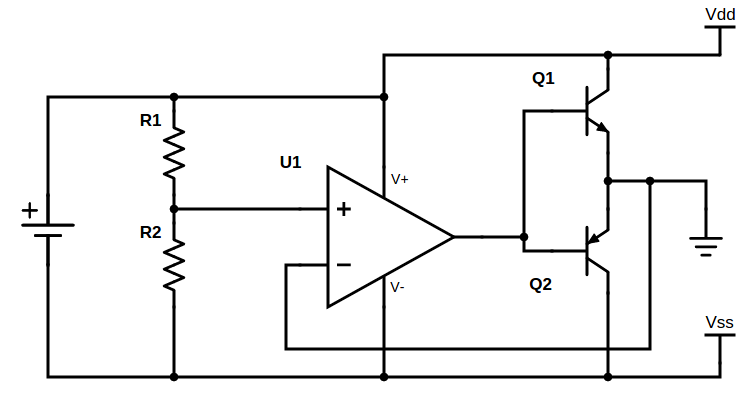
\includegraphics[scale=0.5]{img/fonte.png}
    \caption{Circuito para transformação de fonte assimétrica em simétrica com tera virtual.}
    \label{f_fonte}
\end{figure}

\subsection{Oscilador}
Para o amplificador U1 da figura \ref{f_sensor}, temos que 
\[
V_a = -\frac{\frac{1}{sC_1}}{R_1}V_b = -\frac{1}{sR_1C_1}Vb = -\frac{1}{R_1C_1} \int_{0}^{T}V_b(t)dt.
\]

Para $V_b(t) = cte.$, temos que 

\begin{equation}
V_a = -\frac{V_b}{R_1C_1}T.
\label{e_va}  
\end{equation}

No caso do amplificador U2,

\[
\frac{V_a - V_+}{R_2} = \frac{V_+ - V_b}{R_3} \quad \therefore \quad \frac{V_a}{R_2} - \frac{V_+}{R_2} = \frac{V_+}{R_3} - \frac{V_b}{R_3}
\]

e

\[
\frac{V_a}{R_2} + \frac{V_b}{R_3} = V_+ \bigg (\frac{1}{R_2} + \frac{1}{R_3} \bigg).
\]

Então, 

\[
    V_+ = \frac{V_aR_3 + V_bR_2}{R_3+R_2}.
\]


Assim, se $V_b = -V_{cc}$, $V_b$ irá para $+V_{cc}$ quando $V_+ = 0$, ou seja, quando $V_aR_3 = -V_bR_2$. Logo,

\[ V_a = -V_b\frac{R_2}{R_3} = +V_{cc}\frac{R_2}{R_3}. \]

Isso quer dizer que quando $V_a = +V_{cc}\frac{R_2}{R_3}$, $V_b$ passa de $-V_{cc}$ para $+V_{cc}$. De forma semelhante. pode ser demonstrado que, quando $V_a = -V_{cc}\frac{R_2}{R_3}$, $V_b$ passa de $+V_{cc}$ para $-V_{cc}$.

Portanto, definimos que, para o semiciclo positivo, temos

\begin{equation}
V_a = +V_{cc}\frac{R_2}{R_3},
\label{e_positivo}
\end{equation}

e para o semiciclo negativo

\begin{equation}
V_a = -V_{cc}\frac{R_2}{R_3}.
\label{e_negativo}
\end{equation}

Substituindo a equação \ref{e_va} em \ref{e_positivo},

\[
-\frac{-V_{cc}}{R_1C_1}T_1 = +V_{cc}\frac{R_2}{R_3}
\]

\[
    \therefore T_1 = \bigg ( \frac{R_2}{R_3}R_1\bigg )C_1
\]

e como $T = 4T_1$,

\begin{equation}
T =  4 \frac{R_2}{R_3} R_1C_1.
\label{e_periodo}
\end{equation}


\begin{figure}[H]
    \centering
    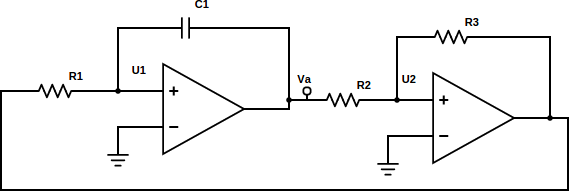
\includegraphics[scale=0.5]{img/sensor.png}
    \caption{Oscilador com amplificadores operacionais.}
    \label{f_sensor}
\end{figure} 

